%!TEX root = karen.tex

\chapter{Keeneland Results}

\authnote{Show plots from paper as "before" and this as after} 

The benchmarks in our first paper (\cite{BolligFlyerErlebacher2012}) demonstrated the initial strong scaling of our implementation for a distributed RK4 iteration and primitive communication with blocking MPI\_send/MPI\_recv routines. Data was acquired on the multi-GPU cluster named Keeneland \cite{Vetter2011}. The scaling of our implementation in the paper was poor as processes regularly waited on communication. However, the objective in \cite{BolligFlyerErlebacher2012} was not to present a well tuned distributed GPU implementation of RBF-FD, but instead focused on the design decisions for partitioning, index mapping, etc. and verification of both single and distributed GPU implementations as inefficient as they were. 

The following data, also acquired on Keeneland, demonstrates performance of our implementation with communication managed by an MPI\_alltoallv collective. The test case considered is the cosine bell advection problem from Section~\ref{sec:cosine_bell}. 

\begin{figure}
\centering
\begin{subfigure}[t]{0.425\textwidth}
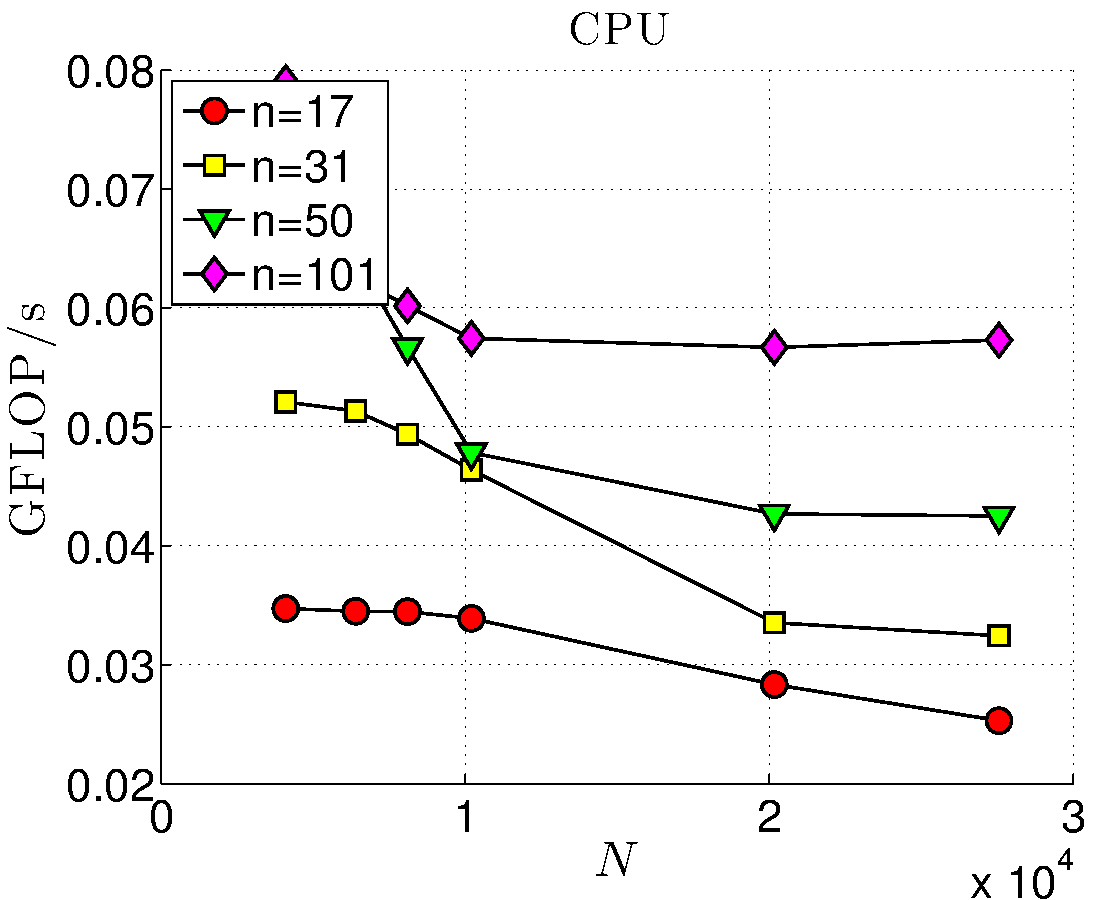
\includegraphics[width=1.0\textwidth]{../figures/keeneland_results/alltoallv/gflops_cpu_1proc_oneWarpPerStencil-eps-converted-to.pdf}
\caption{One warp per stencil kernel on one GPU in Keeneland}
\label{fig:gflops_cpu_1proc_keeneland}
\end{subfigure} 

\begin{subfigure}[t]{0.425\textwidth}
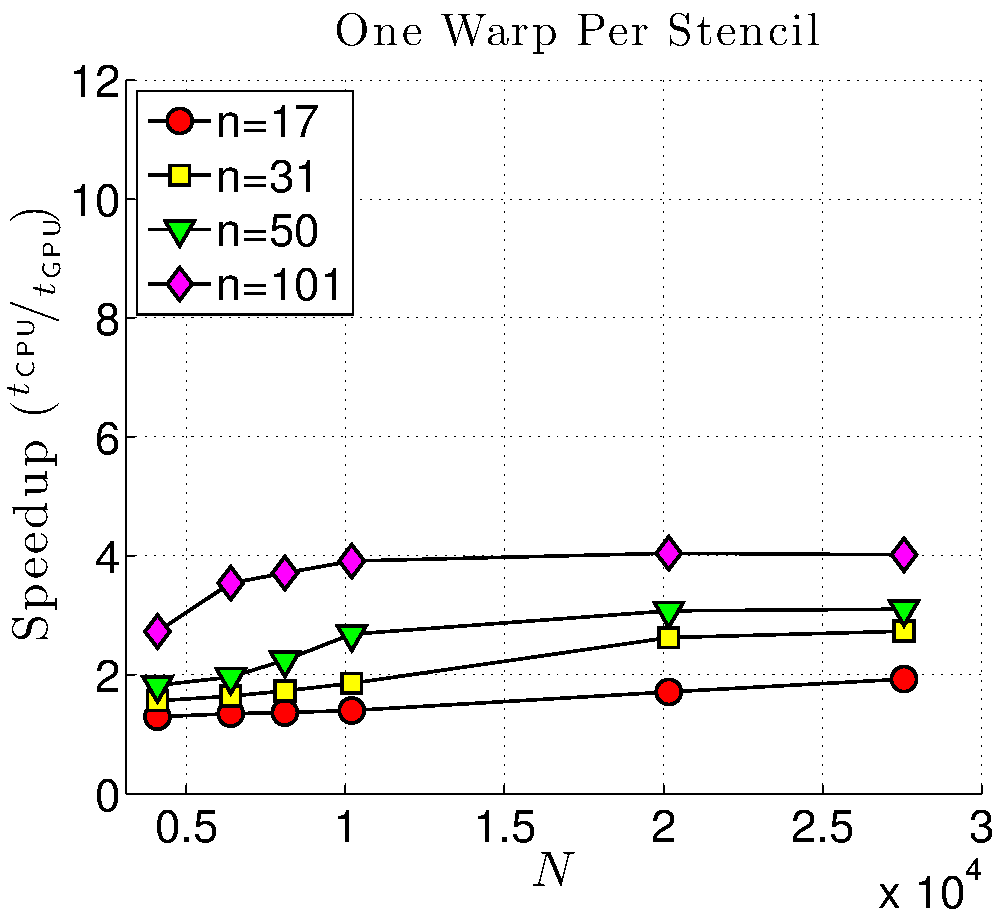
\includegraphics[width=1.0\textwidth]{../figures/keeneland_results/alltoallv/speedup_1proc_oneWarpPerStencil-eps-converted-to.pdf}
\caption{One warp per stencil kernel on one GPU in Keeneland}
\label{fig:speedup_1proc_oneWarp_keeneland}
\end{subfigure} 
\begin{subfigure}[t]{0.425\textwidth}
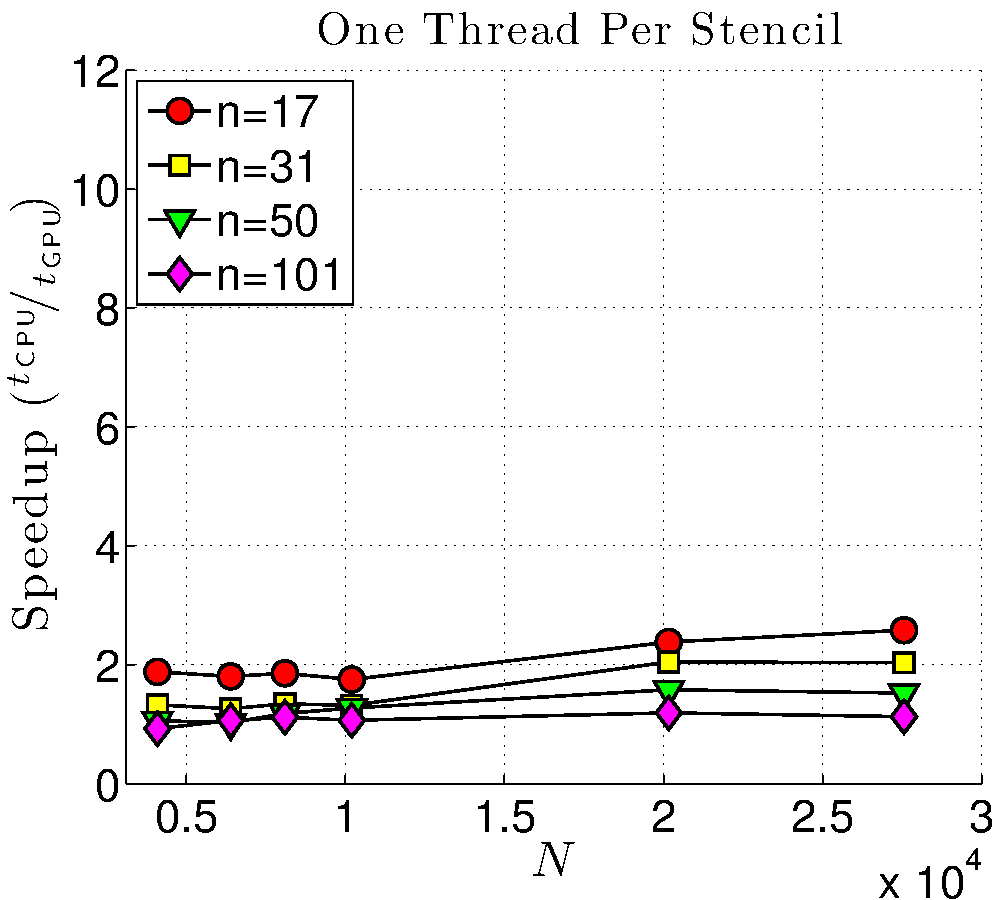
\includegraphics[width=1.0\textwidth]{../figures/keeneland_results/alltoallv/speedup_1proc_oneThreadPerStencil-eps-converted-to.pdf}
\caption{One warp per stencil kernel on one GPU in Keeneland}
\label{fig:speedup_1proc_oneThread_keeneland}
\end{subfigure} 
\begin{subfigure}[t]{0.425\textwidth}
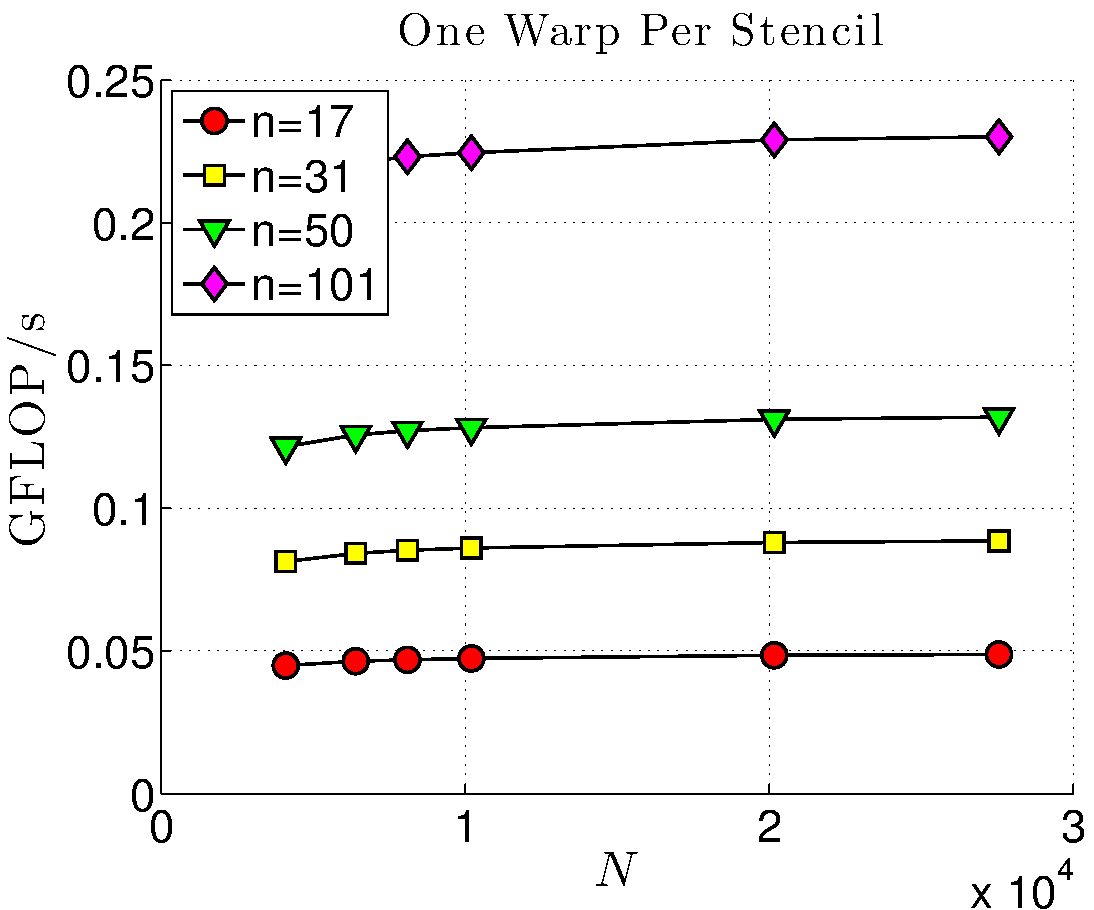
\includegraphics[width=1.0\textwidth]{../figures/keeneland_results/alltoallv/gflops_gpu_1proc_oneWarpPerStencil-eps-converted-to.pdf}
\caption{One warp per stencil kernel on one GPU in Keeneland}
\label{fig:gflops_gpu_1proc_oneWarp_keeneland}
\end{subfigure} 
\begin{subfigure}[t]{0.425\textwidth}
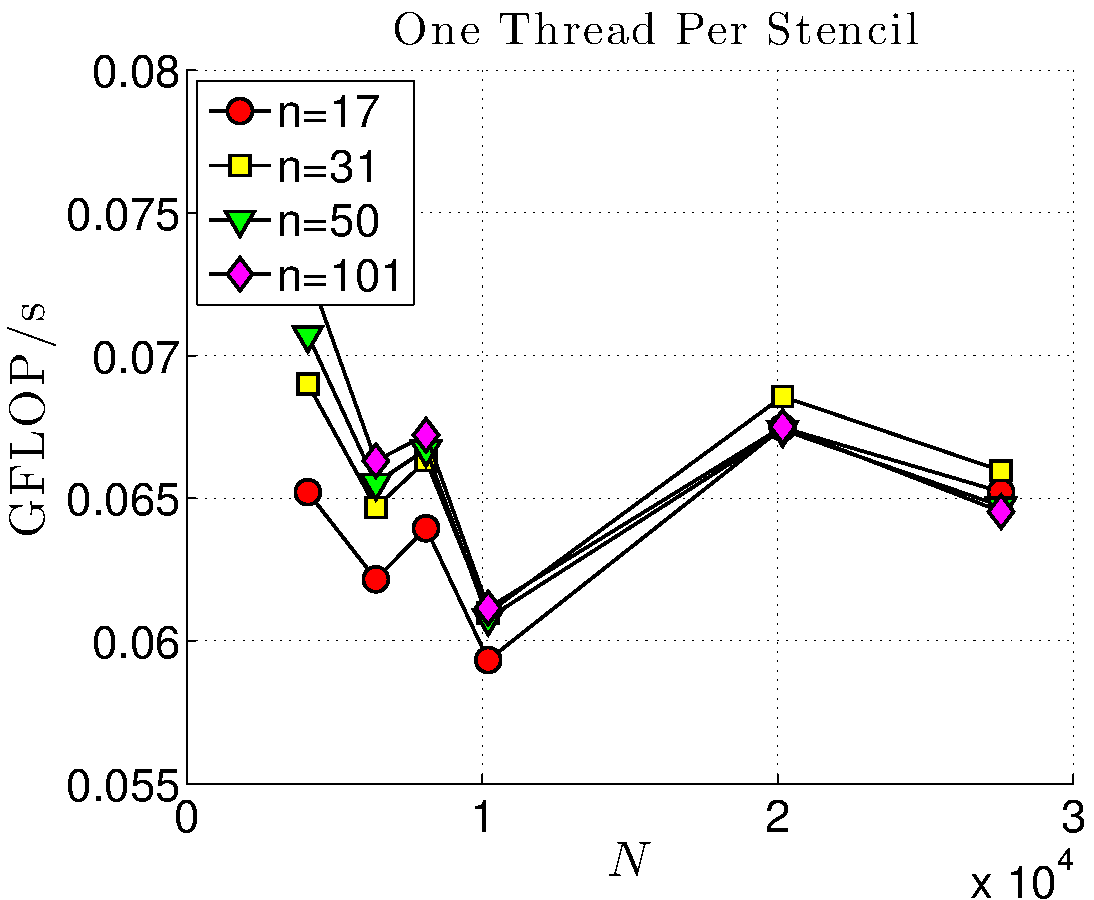
\includegraphics[width=1.0\textwidth]{../figures/keeneland_results/alltoallv/gflops_gpu_1proc_oneThreadPerStencil-eps-converted-to.pdf}
\caption{One warp per stencil kernel on one GPU in Keeneland}
\label{fig:gflops_gpu_1proc_oneThread_keeneland}
\end{subfigure} 
\end{figure} 


\begin{figure}
\centering
\begin{subfigure}[t]{0.425\textwidth}
\centering
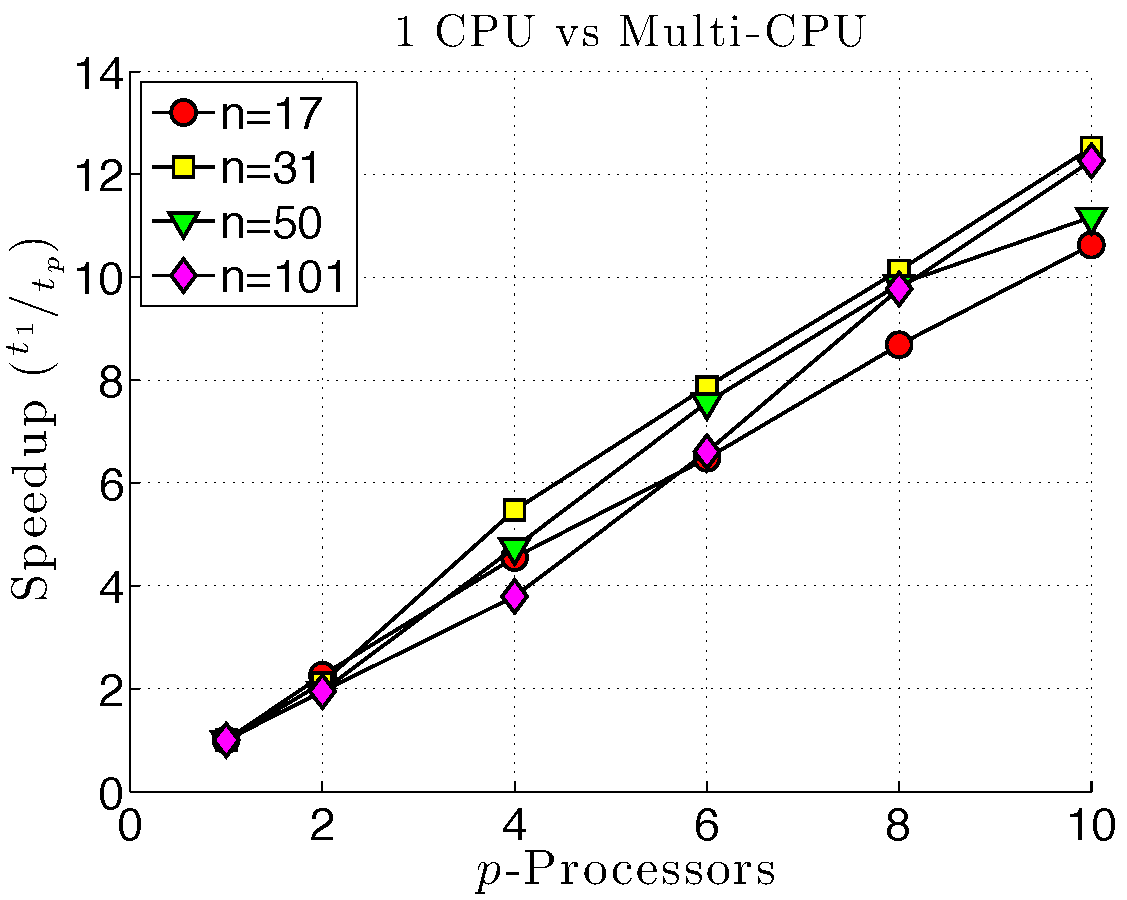
\includegraphics[width=1.0\textwidth]{../figures/keeneland_results/alltoallv/speedup_1CPU_vs_NCPU.pdf}
\caption{Multi-CPU strong scaling on Keeneland for one warp per stencil. Problem size is sufficiently large to hide latency in MPI communication.}
\label{fig:alltoall_multicpu_scaling}
\end{subfigure} 
\begin{subfigure}[t]{0.425\textwidth}
\centering
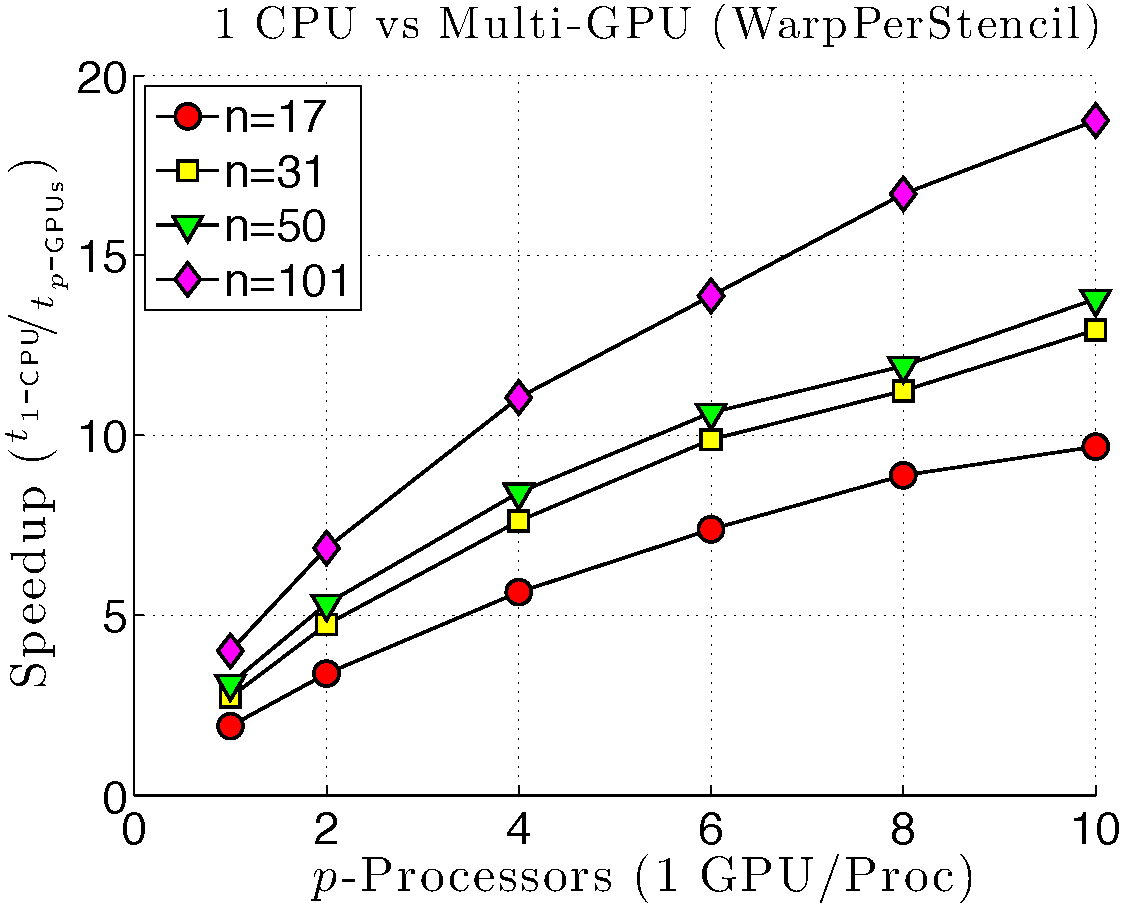
\includegraphics[width=1.0\textwidth]{../figures/keeneland_results/alltoallv/speedup_1CPU_vs_NGPU_WarpPerStencil.pdf}
\caption{Multi-GPU strong scaling vs one CPU on Keeneland for one warp per stencil}
\label{fig:alltoall_multigpu_vs_cpu_scaling}
\end{subfigure} 
\begin{subfigure}[t]{0.425\textwidth}
\centering
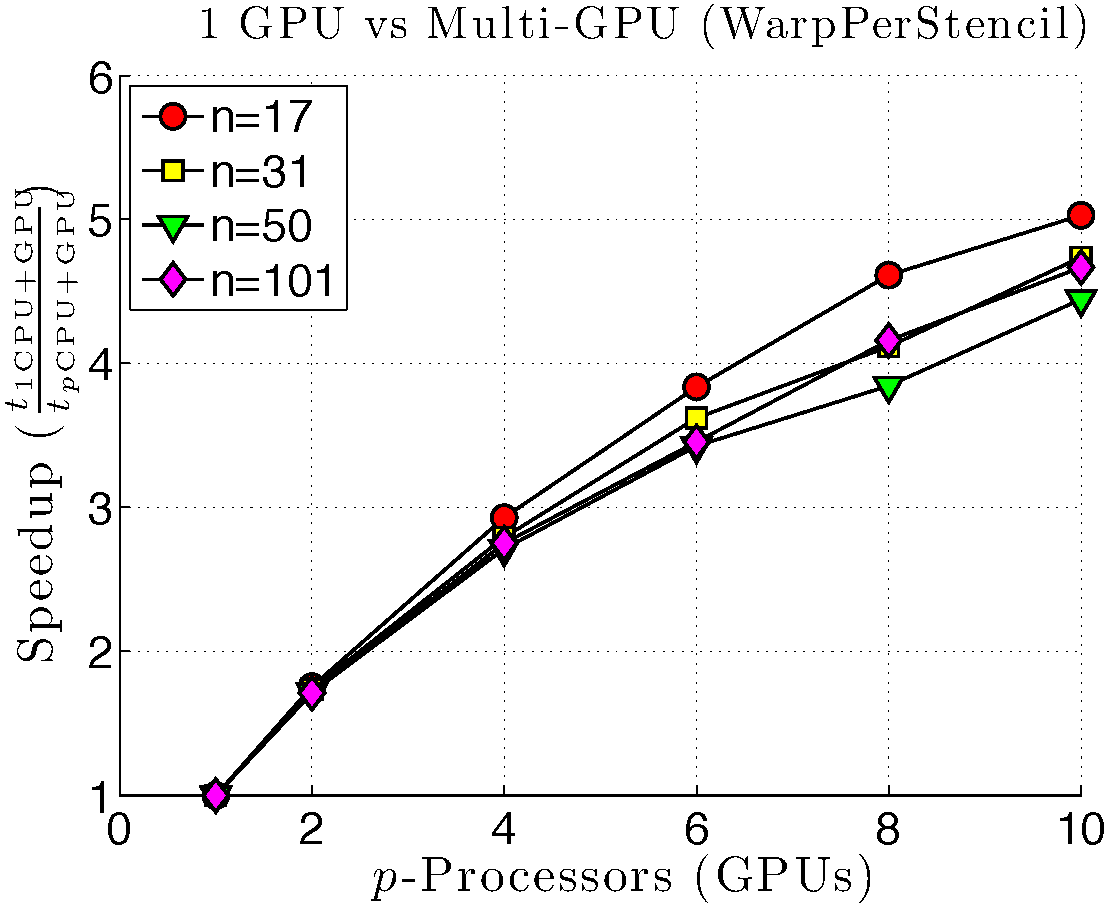
\includegraphics[width=1.0\textwidth]{../figures/keeneland_results/alltoallv/speedup_1GPU_vs_NGPU_WarpPerStencil.pdf}
\caption{Multi-GPU strong scaling vs one GPU on Keeneland for one warp per stencil}
\label{fig:alltoall_multigpu_vs_gpu_scaling}
\end{subfigure} 
\end{figure}

\begin{figure}
\centering
\begin{subfigure}[t]{0.425\textwidth}
\centering
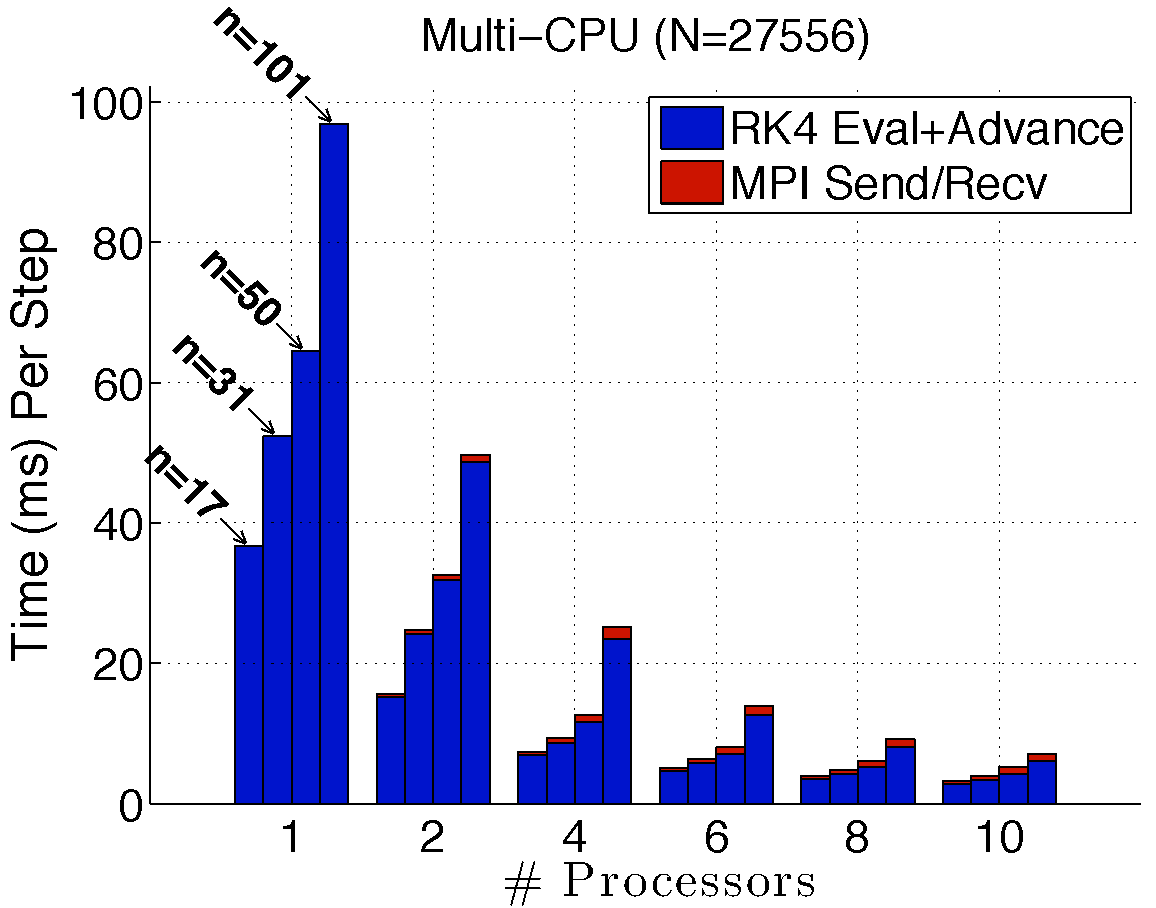
\includegraphics[width=1.0\textwidth]{../figures/keeneland_results/alltoallv/multiCPU_costs.pdf}
\caption{Multi-CPU benchmarks by component on Keeneland}
\label{fig:alltoall_multicpu_costs}
\end{subfigure} 
\begin{subfigure}[t]{0.425\textwidth}
\centering
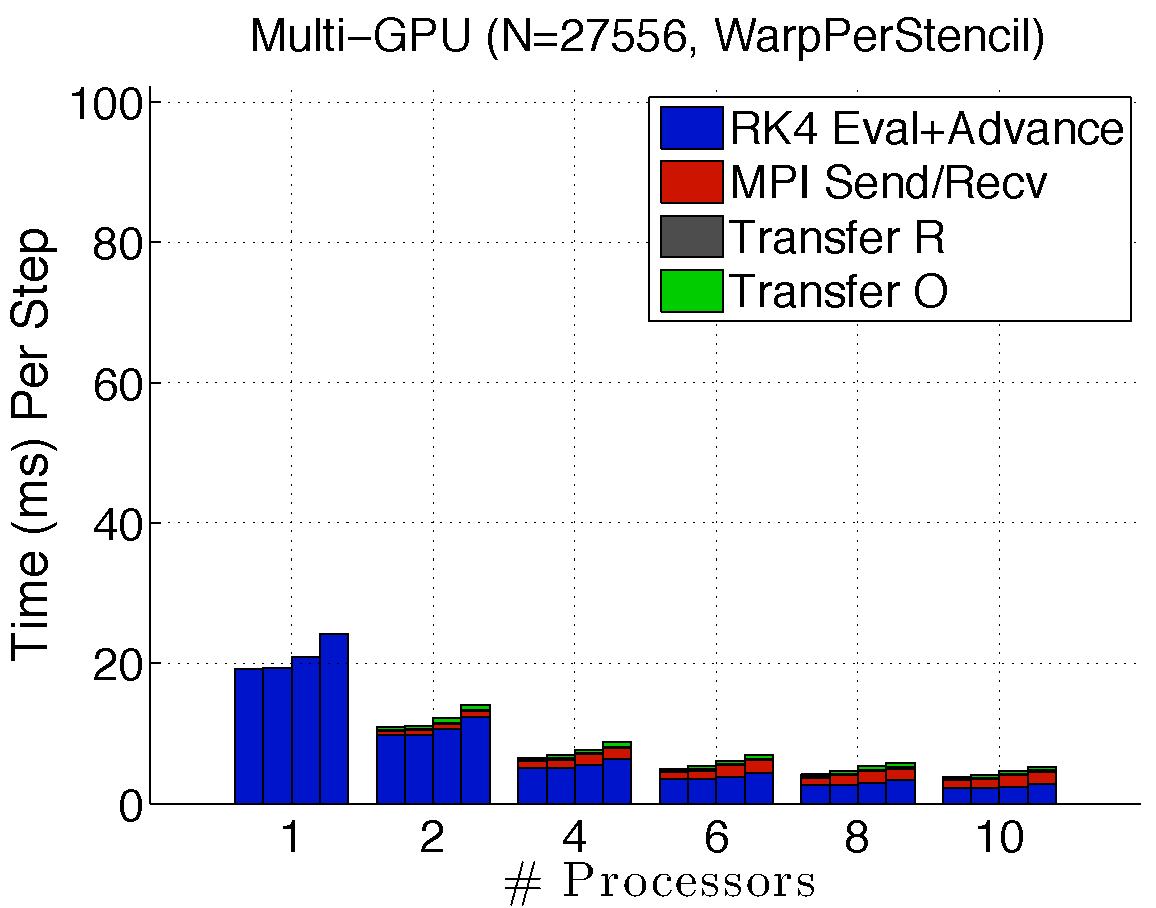
\includegraphics[width=1.0\textwidth]{../figures/keeneland_results/alltoallv/multiGPU_warp_costs.pdf}
\caption{Multi-GPU benchmarks by component on Keeneland}
\label{fig:alltoall_multigpu_costs}
\end{subfigure} 
\end{figure} 

%TODO: urgent
\authnote{Relocate SpMV only data:} 
Figure~\ref{fig:alltoall_1proc_warp} shows the speedup gained of the one warp-per-stencil GPU kernel

Figure~\ref{fig:alltoall_multicpu_scaling}  shows the strong scalability of our method on Multiple CPUs. In distributed computing, ideal scaling is linear. This figure demonstrates that our method does scale linearly (almost super-linearly) as the number of CPUs increases, so our prospect for spanning all CPUs on Keeneland is within reach for problem sizes large enough. The super-linear speedup seen for 10 processors results from improved caching on processors as their individual problem sizes decrease and the processors are able to keep a larger percentage of the problem within fast cache memory.

Figure~\ref{fig:alltoall_multigpu_vs_cpu_scaling}  shows the scaling of multiple GPUs vs 1 CPU. Ideally, this figure would be the product of the previous two figures since the GPUs are attached to CPUs in a one to one correspondence. However, we see from the sub-linear scaling that while the GPU accelerators are decreasing the time to compute solutions, there is less and less return of investment as the number of processors increase. Between this Figure and the previous, the only thing that differs is the hardware on which stencils are evaluated. The cost of communication stays the same as in the previous figure. But that means the communication consumes a increasing percentage of the iteration time, until is dominates. 
Additionally, computing on the GPU requires transfer (additional communication) of data between CPU and GPU. 

Figure~\ref{fig:alltoall_multigpu_vs_gpu_scaling} shows the scalability of multiple GPUs vs 1 GPU. Here we see a sub-linear behavior for all cases. This is attributed to both the cost of transfer between CPUs and GPUs and the decreasing problem size as number of processors increases, which underutilizes the GPUs. 


Figure~\ref{fig:alltoall_multicpu_costs} and Figure~\ref{fig:alltoall_multigpu_costs} show the smaller percentage of time per iteration dedicated to communication compared to the figures in the paper. In the Figure~\ref{fig:alltoall_multigpu_costs}, the way the times bottom out indicates we are/have converged on the minimum time required to launch a GPU kernel, transfer to/from the GPU, and communicate the problem via MPI. To scale to more processors, a larger problem size is absolutely necessary.


%I am generating another set of figures that demonstrate the scaling when we overlap communication and computation. MPI collectives do not allow overlap, but the asynchronous GPU kernel launches do. Therefore, I expect:
%    - the scaling on multiple CPUs vs 1 CPU to be the same as it is now
%    - the scaling on multiple GPUs vs 1 GPU will improve to linear/super-linear for problem sizes that occupy the hardware longer than the minimum kernel launch time. For N=27556 we might only see linear speedup up to 6 or 8 processors. 
%    - larger problem sizes will still be necessary (I have benchmarks for 100K, 500K and 1M on the sphere).
%    

%TODO: Work-Group Size and Number of Stencils
%What if a work-group is larger than a warp? What if the group was occupied by multiple stencils. What improvements to speedup do we see?
%
%How many stencils can each group handle (assuming values stay in shared memory? 
%Shared memory bank conflicts? How do we sort the values? 
%What is the occupancy of the GPU?
%


\chapter{Spear Results}

These results were run on Spear. MPI communication is done with an MPI\_alltoallv collective. The test case is the vortex roll-up. 

\begin{figure}[htbp]
\centering
\begin{subfigure}[b]{0.425\textwidth}
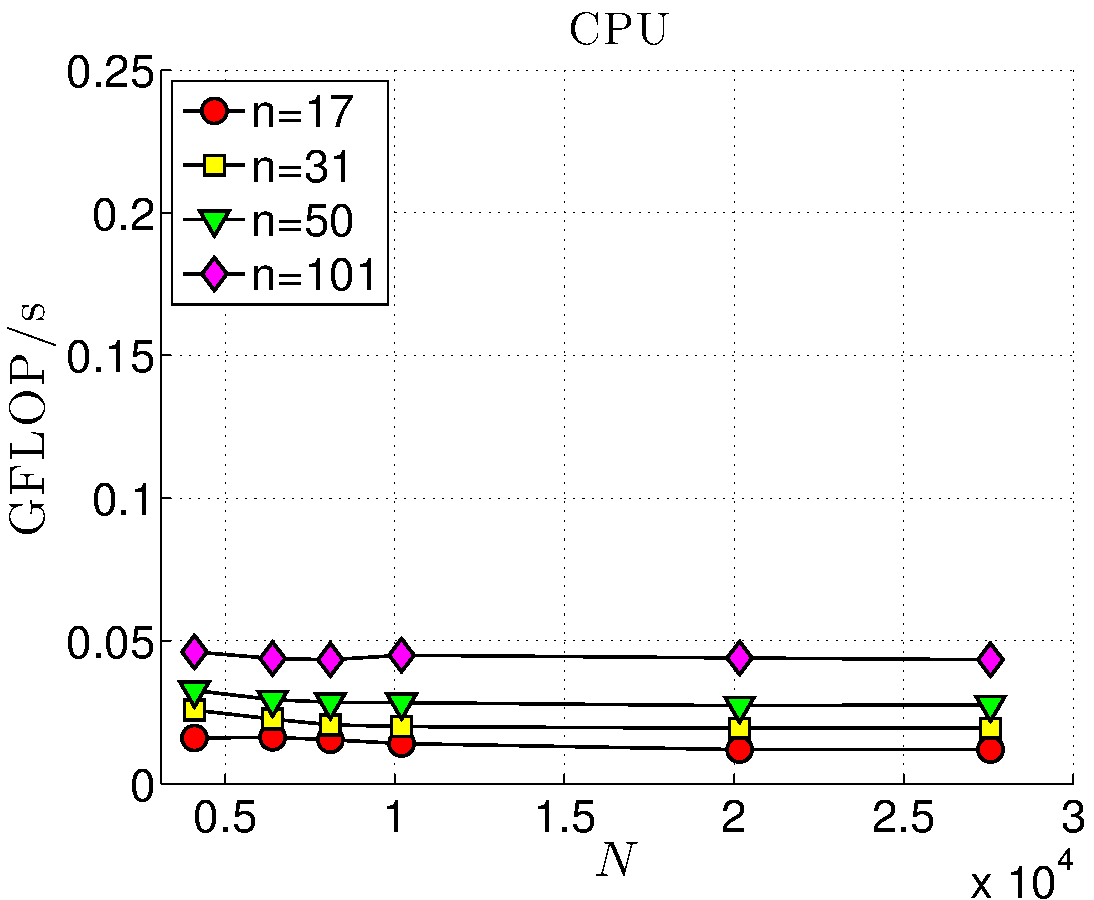
\includegraphics[width=1.0\textwidth]{../figures/spear_results/vortex/gflops_cpu_1proc_oneWarpPerStencil-eps-converted-to.pdf}
\caption{One warp per stencil kernel on one GPU in Spear}
\label{fig:alltoall_1proc_warp}
\end{subfigure} 

\begin{subfigure}[b]{0.425\textwidth}
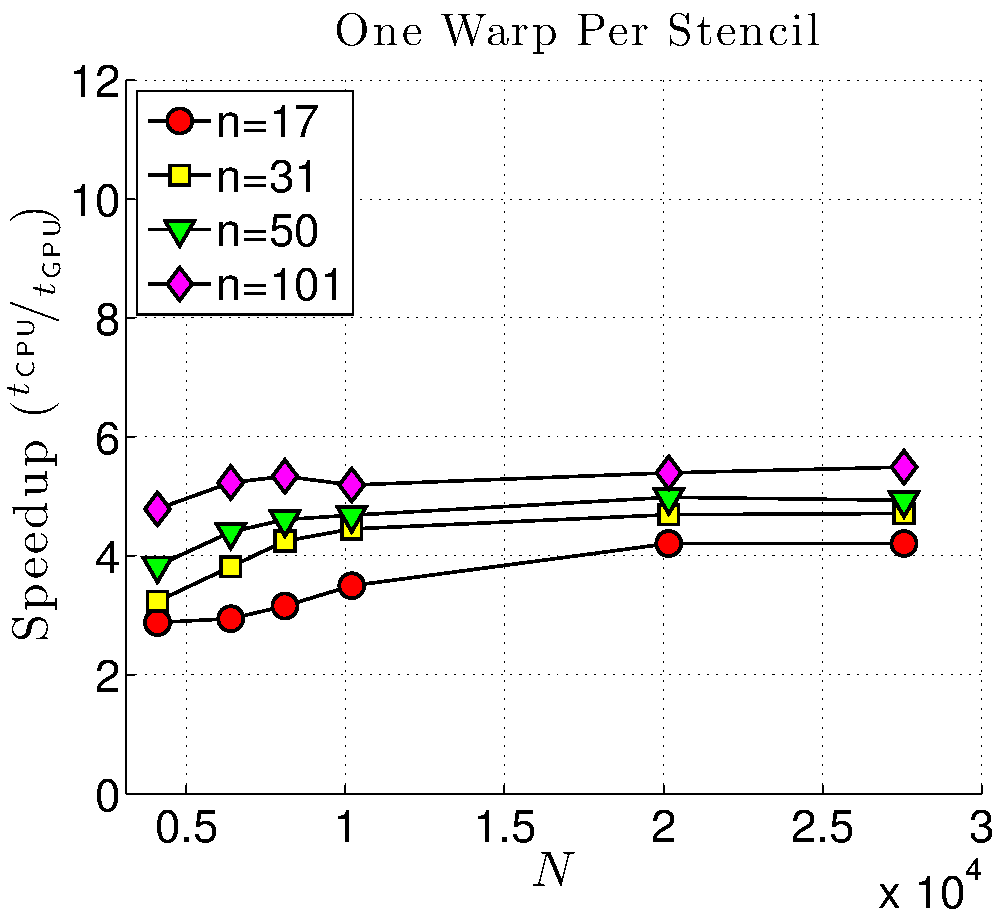
\includegraphics[width=1.0\textwidth]{../figures/spear_results/vortex/speedup_1proc_oneWarpPerStencil-eps-converted-to.pdf}
\caption{One warp per stencil kernel on one GPU in Spear}
\label{fig:alltoall_1proc_warp}
\end{subfigure} 
\begin{subfigure}[b]{0.425\textwidth}
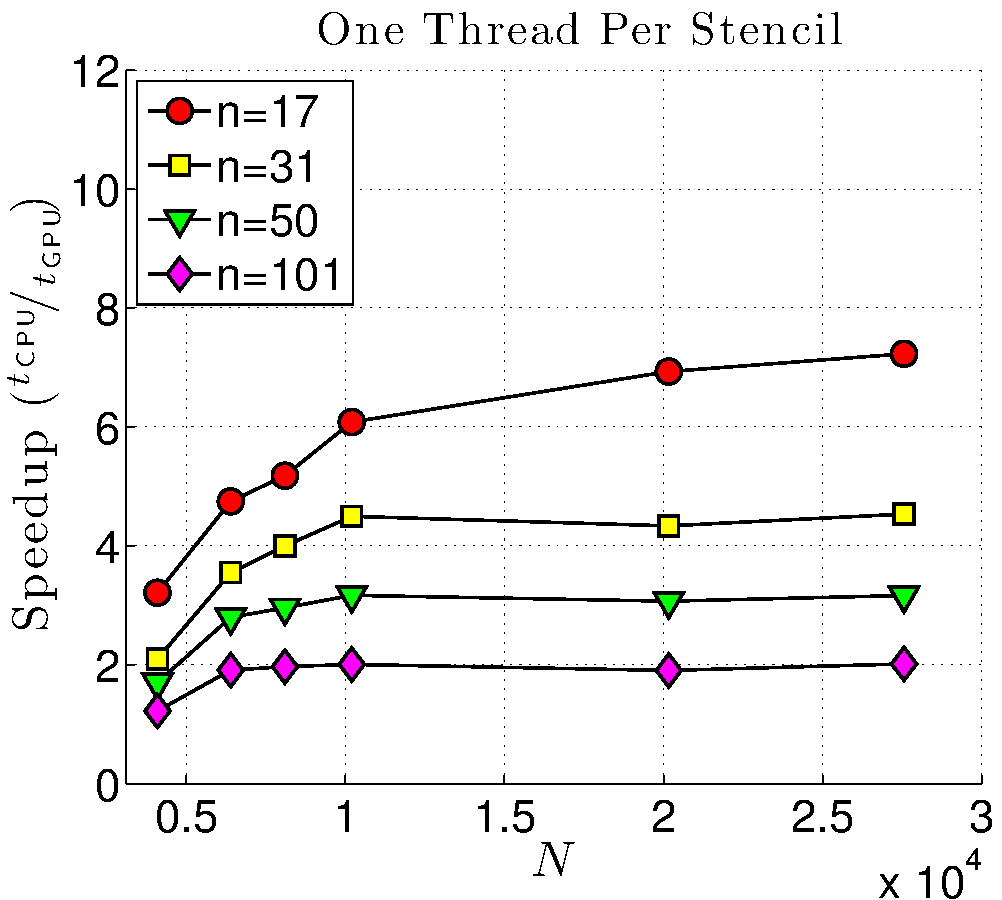
\includegraphics[width=1.0\textwidth]{../figures/spear_results/vortex/speedup_1proc_oneThreadPerStencil-eps-converted-to.pdf}
\caption{One warp per stencil kernel on one GPU in Spear}
\label{fig:alltoall_1proc_warp}
\end{subfigure} 
\begin{subfigure}[b]{0.425\textwidth}
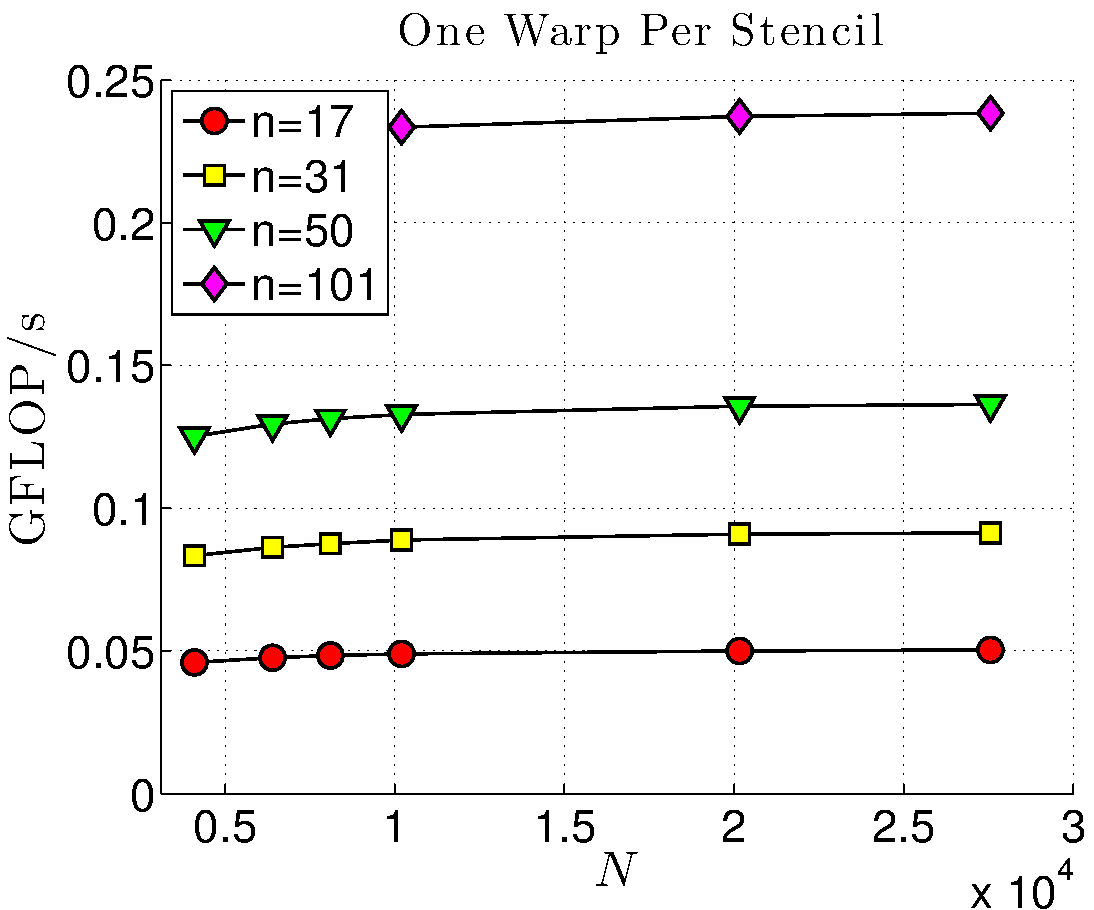
\includegraphics[width=1.0\textwidth]{../figures/spear_results/vortex/gflops_gpu_1proc_oneWarpPerStencil-eps-converted-to.pdf}
\caption{One warp per stencil kernel on one GPU in Spear}
\label{fig:alltoall_1proc_warp}
\end{subfigure} 
\begin{subfigure}[b]{0.425\textwidth}
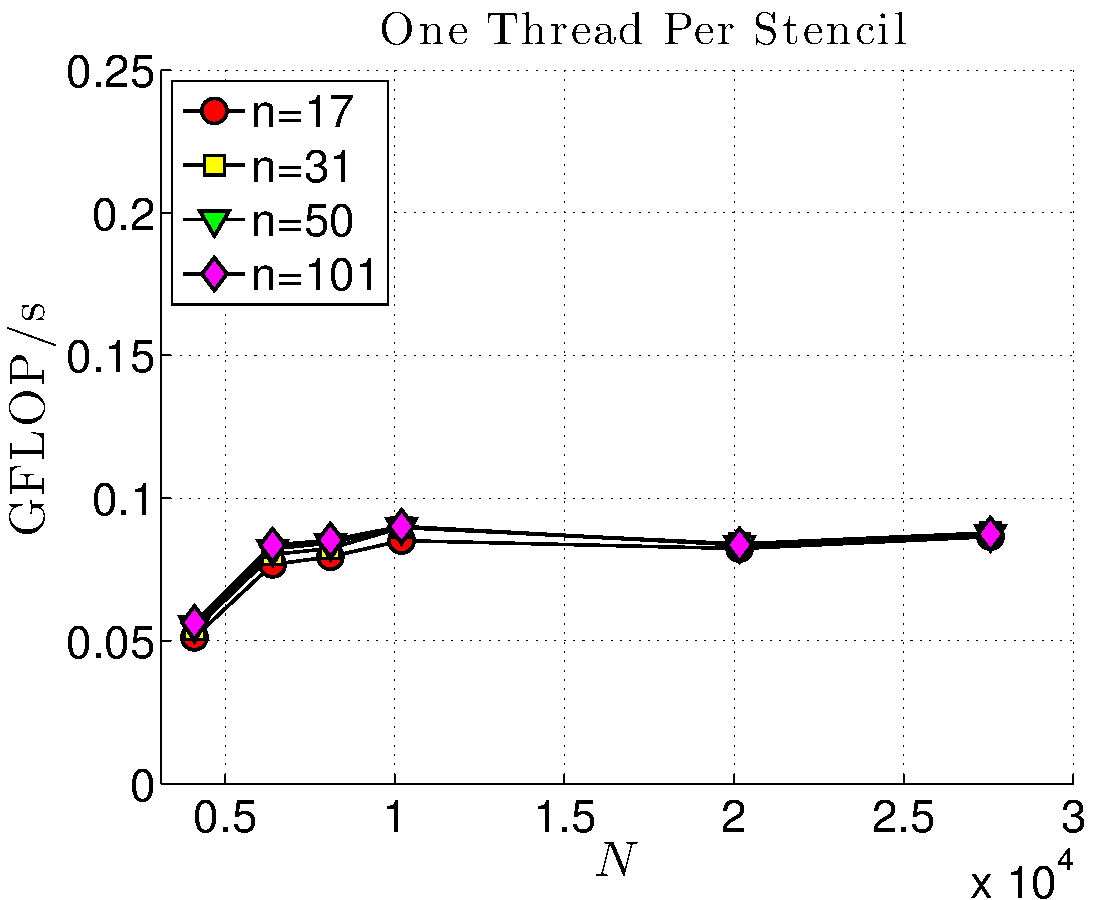
\includegraphics[width=1.0\textwidth]{../figures/spear_results/vortex/gflops_gpu_1proc_oneThreadPerStencil-eps-converted-to.pdf}
\caption{One warp per stencil kernel on one GPU in Spear}
\label{fig:alltoall_1proc_warp}
\end{subfigure} 
\end{figure}

\begin{figure}[htbp]
\centering
\begin{subfigure}[b]{0.425\textwidth}
\centering
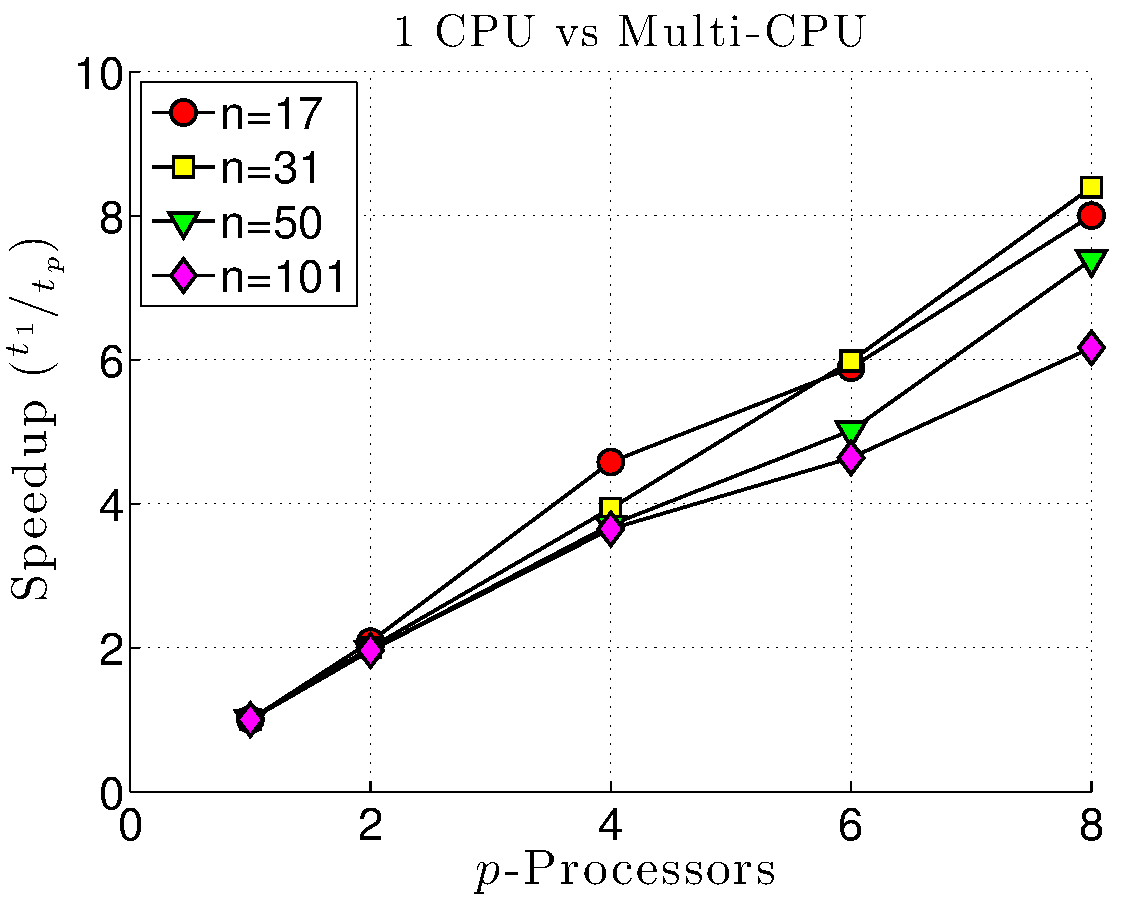
\includegraphics[width=1.0\textwidth]{../figures/spear_results/vortex/speedup_1CPU_vs_NCPU-eps-converted-to.pdf}
\caption{Multi-CPU strong scaling on spear for one warp per stencil}
\label{fig:alltoall_multicpu_scaling}
\end{subfigure} 
\begin{subfigure}[b]{0.425\textwidth}
\centering
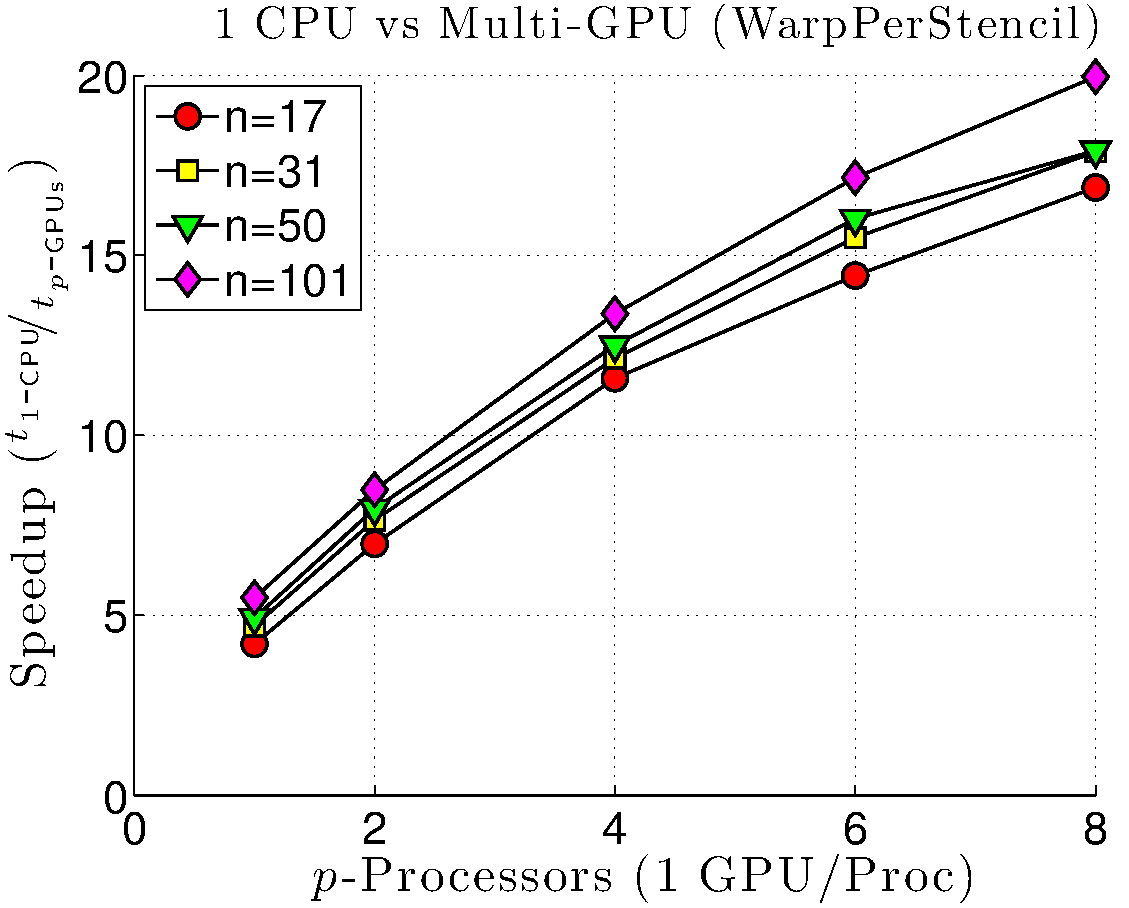
\includegraphics[width=1.0\textwidth]{../figures/spear_results/vortex/speedup_1CPU_vs_NGPU_WarpPerStencil-eps-converted-to.pdf}
\caption{Multi-GPU strong scaling vs one CPU on Spear for one warp per stencil}
\label{fig:alltoall_multigpu_vs_cpu_scaling}
\end{subfigure} 
\begin{subfigure}[b]{0.425\textwidth}
\centering
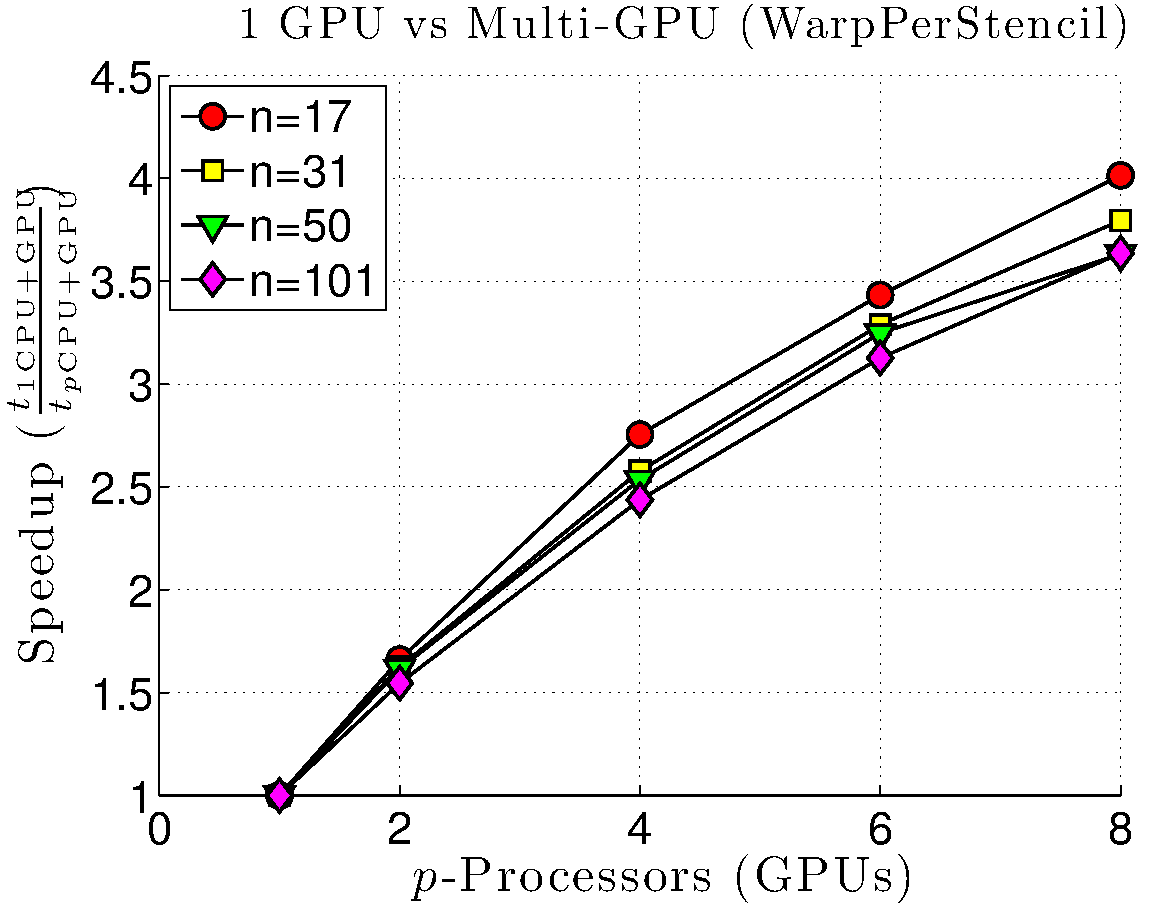
\includegraphics[width=1.0\textwidth]{../figures/spear_results/vortex/speedup_1GPU_vs_NGPU_WarpPerStencil-eps-converted-to.pdf}
\caption{Multi-GPU strong scaling vs one GPU on Spear for one warp per stencil}
\label{fig:alltoall_multigpu_vs_gpu_scaling}
\end{subfigure} 
\end{figure} 


\section{Spear SpMV} 

\begin{figure}[htbp]
\centering
\begin{subfigure}[b]{0.425\textwidth}
\centering
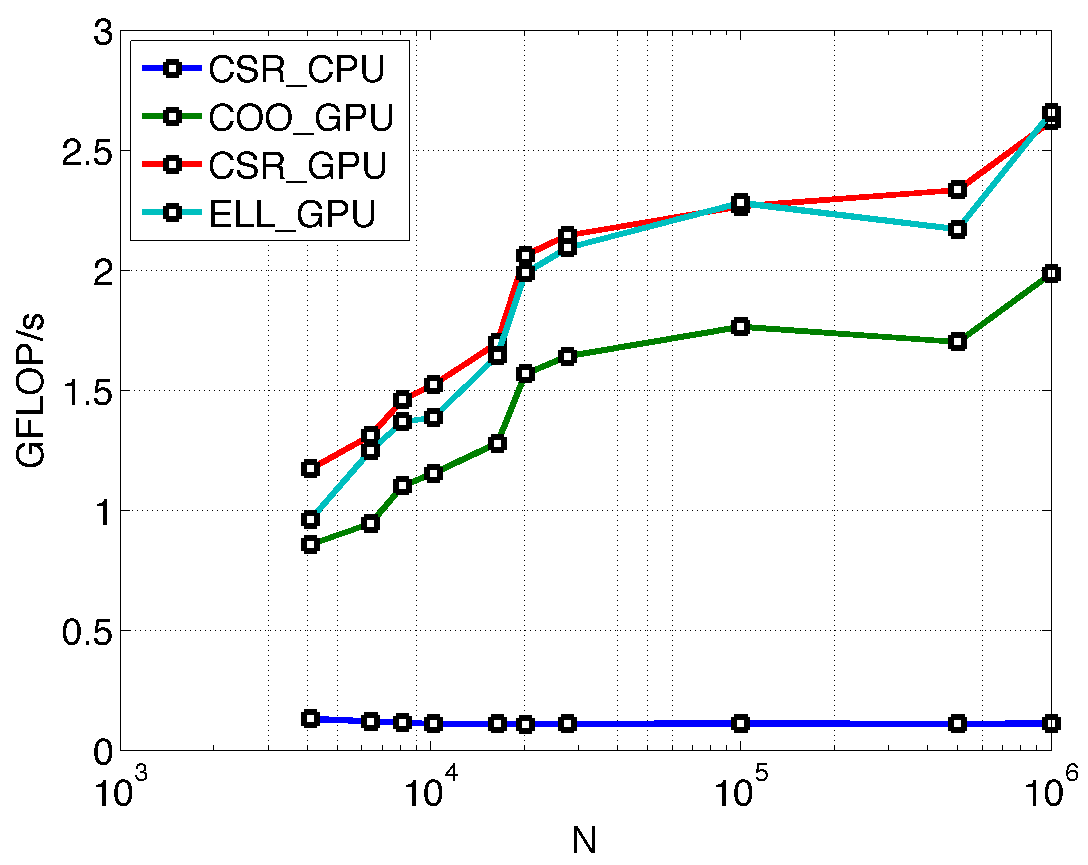
\includegraphics[width=1.0\textwidth]{../figures/spear_results/spmv/spmv_vcl_gflops-eps-converted-to.pdf}
\caption{Multi-CPU strong scaling on spear for one warp per stencil}
\label{fig:alltoall_multicpu_scaling}
\end{subfigure} 
\begin{subfigure}[b]{0.425\textwidth}
\centering
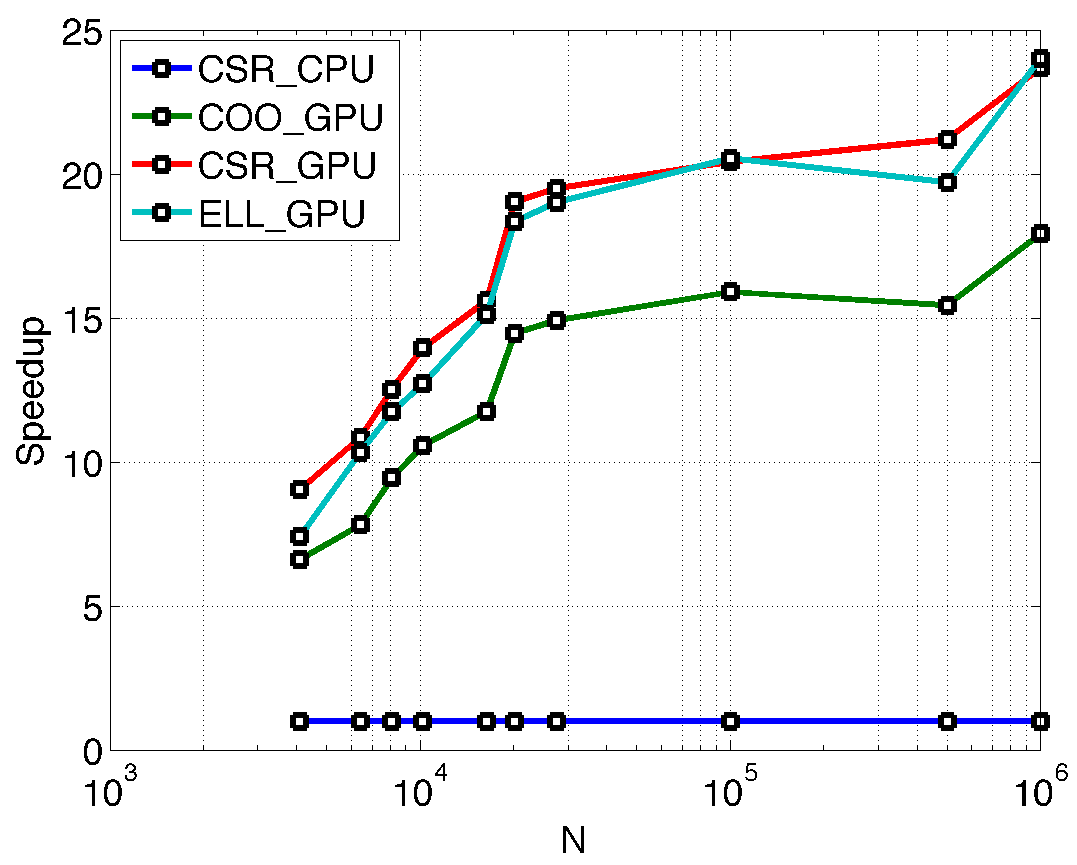
\includegraphics[width=1.0\textwidth]{../figures/spear_results/spmv/spmv_vcl_speedup-eps-converted-to.pdf}
\caption{Multi-GPU strong scaling vs one CPU on Spear for one warp per stencil}
\label{fig:alltoall_multigpu_vs_cpu_scaling}
\end{subfigure} 
\end{figure}
